
\begin{section}{Approach}
\label{sec:approach}
In this section we describe the framework for detection of sensor attacks for systems with unknown or changing dynamics and adaptive motion planning to solve Problems \ref{problem1} and \ref{problem2} to guarantee vehicle safety. We follow the architecture in the block diagrams of Fig. \ref{fig:system_arch} to accomplish these problems. A detector monitors sensor measurements and calculated inputs for sensor attacks, which allows an uncompromised input $u(k)$ to control the system. At the same time, the position estimator along with the high level motion planner update the reference $r(k)$ to the controller to ensure safety.

\begin{figure}[ht!]
\vspace{1pt}
\centering
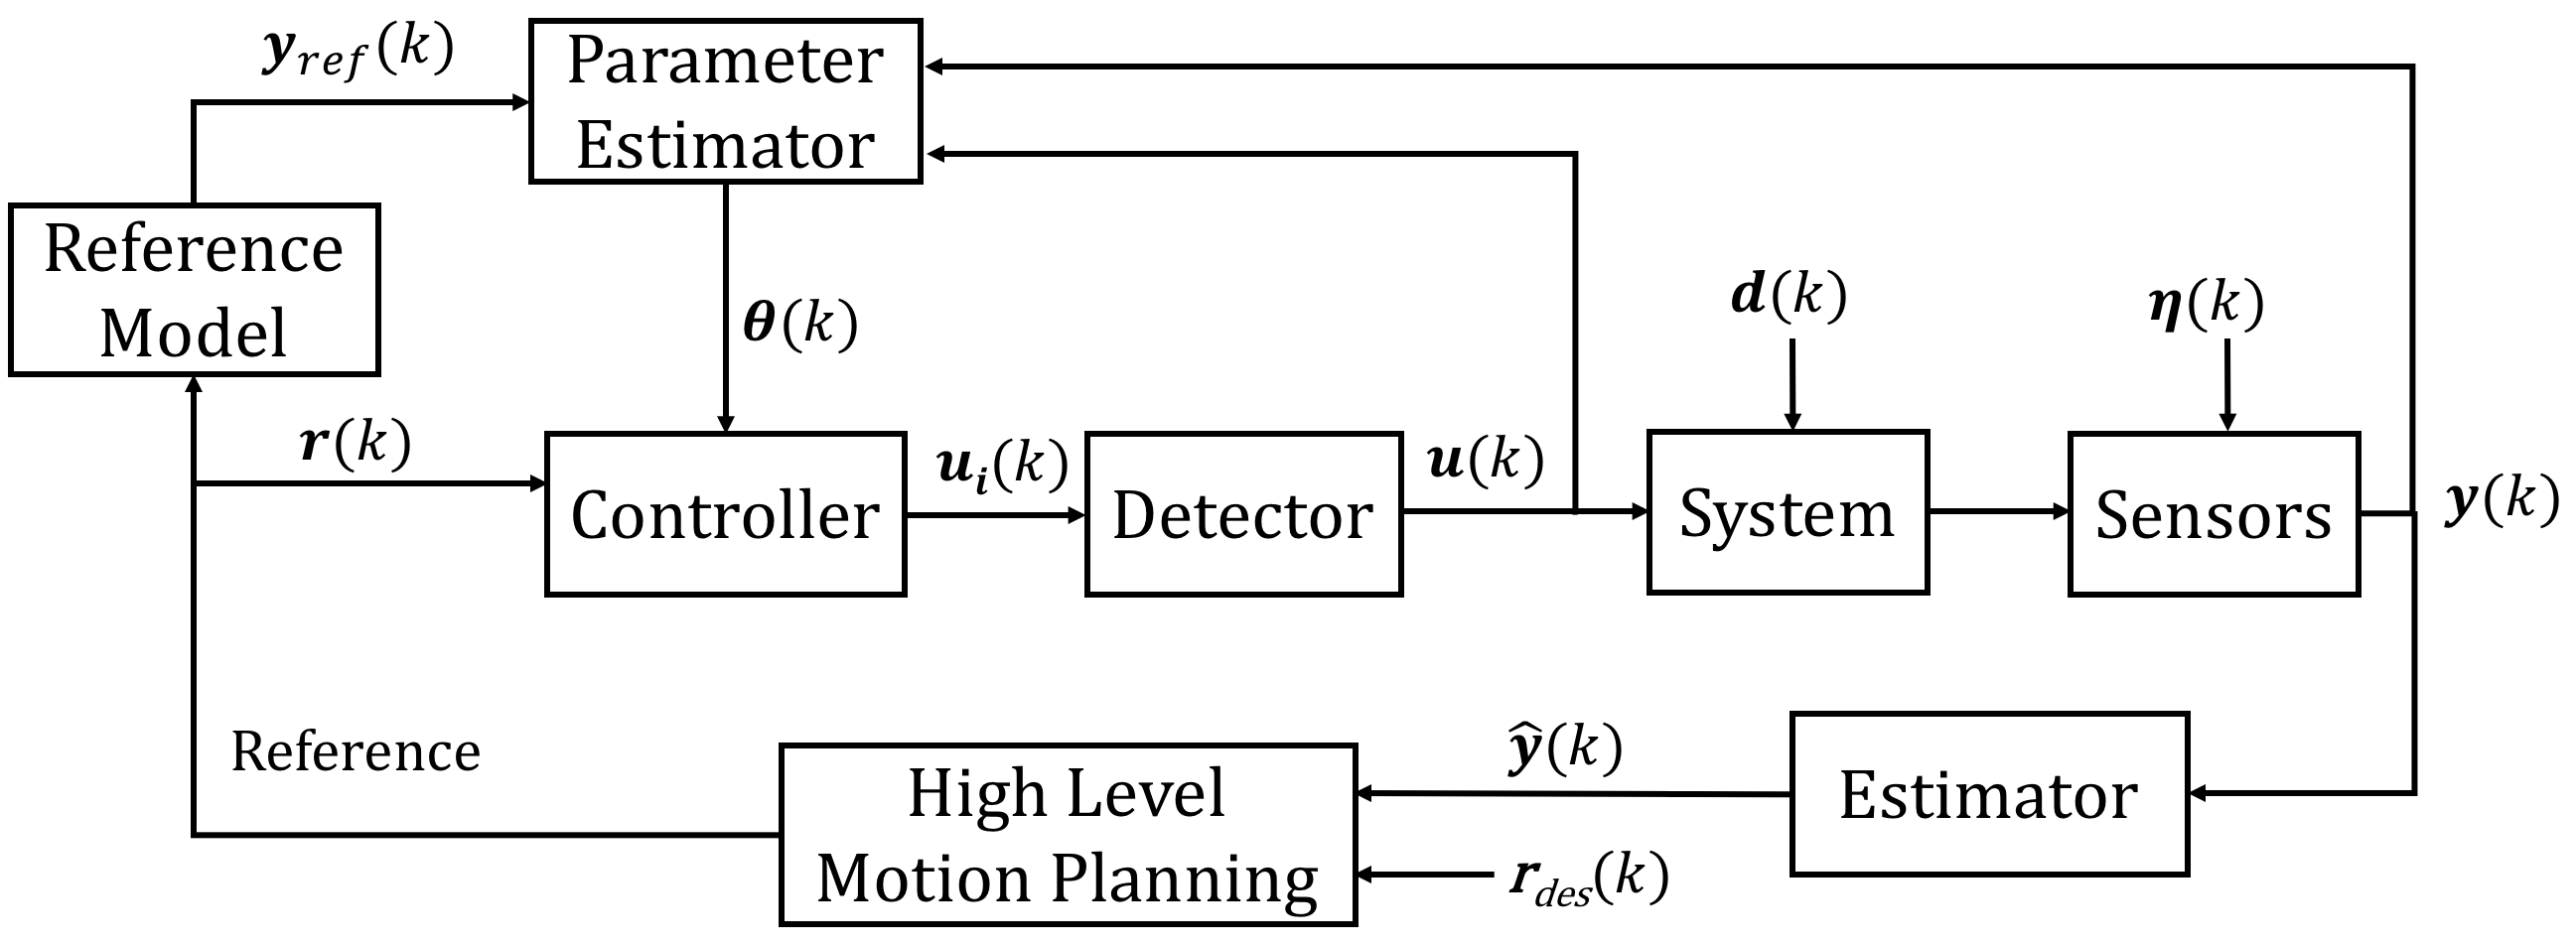
\includegraphics[width=0.46\textwidth]{sys_arch.png}
\caption{Overall system architecture showing the relationship between the reference model adaptive controller and the adaptive motion planner.}
\label{fig:system_arch}
\end{figure}

\subsection{Resilient Adaptive Control}
\label{sec:Res_adapt_control}

A Resilient Adaptive Controller will allow the system to detect sensor attacks while maintaining control performance as dynamical and disturbance uncertainties occur. To maintain this control performance, a Model Reference Adaptive Controller is used. First, we want to ensure adequate information of the system is known in order to design the resilient adaptive controller, the following assumptions need to be true:
	\begin{enumerate}[leftmargin=3\parindent]
	\item[$A1)$] all zeros of $B^{'}(z^{-1})z^q$ from \eqref{eq:B_prime} are within $|z|<1$. 
	\item[$A2)$] $p$ and $q$ are known. 
	\item[$A3)$] the system delay $d$ is known.
	\item[$A4)$] all poles of $E(z^{-1})z^w$ from \eqref{eq:reference model_z} are within $|z|<1$.
	\end{enumerate}
The zeros $z$ of the system are within the discrete $z-plane$ while $p$, $q$, and $d$ are the dimensions of \eqref{eq:transfer_function}. For detection of sensor attacks in dynamically changing or unknown systems, the model reference adaptive control is an effective solution to the problem. We utilize many of the MRAC's assurances and guarantees for our technique to detect sensor attacks when the system model is changing or unknown. We know that under the assumptions of (A1-A4), the following are true \cite{tao2003adaptive},
	\begin{enumerate}[label=(\roman*),leftmargin=3\parindent]
	\label{assumtions_ensure}
	\item[$T1)$] $y(k)$ and $u(k)$ are bounded 
	\item[$T2)$] $\lim_{k\to\infty}(y(k)-y^*(k))=0$
	\label{Truth2}
	\item[$T3)$] $\sum_{k=0}^\infty(y(k)-y^*(k))^2<\infty$
	\end{enumerate}
with $y(k)$ as the system output and $y^*(k)$ is a tracking signal from the reference model. This ensures the system's output asymptotically converges to the reference model's tracking signal in a finite amount of time.

The resilient adaptive controller will employ an architecture of redundant subsystems, as shown in Fig. \ref{fig:det_arch}. Each sensor measurement $y_i$ where $i=1,2,\dots,s$ has its own adaptive controller to generate an input $u^*_i$ to follow a desired tracking signal $y^*_i$. Each of the output sensor measurements, when uncompromised, have convergence (T2) towards their desired tracking signal from the corresponding reference model. 
    \begin{equation}
    \label{multiple_output_tracking}
    \lim_{k\to\infty}(y_i(k)-y^*_i(k))=0, \text{ }\forall i
    \end{equation}
This remains true with a changing reference signal $r_i(k)$, changing dynamics, or bounded disturbances. 

\begin{figure}[ht!]
\vspace{1pt}
\centering
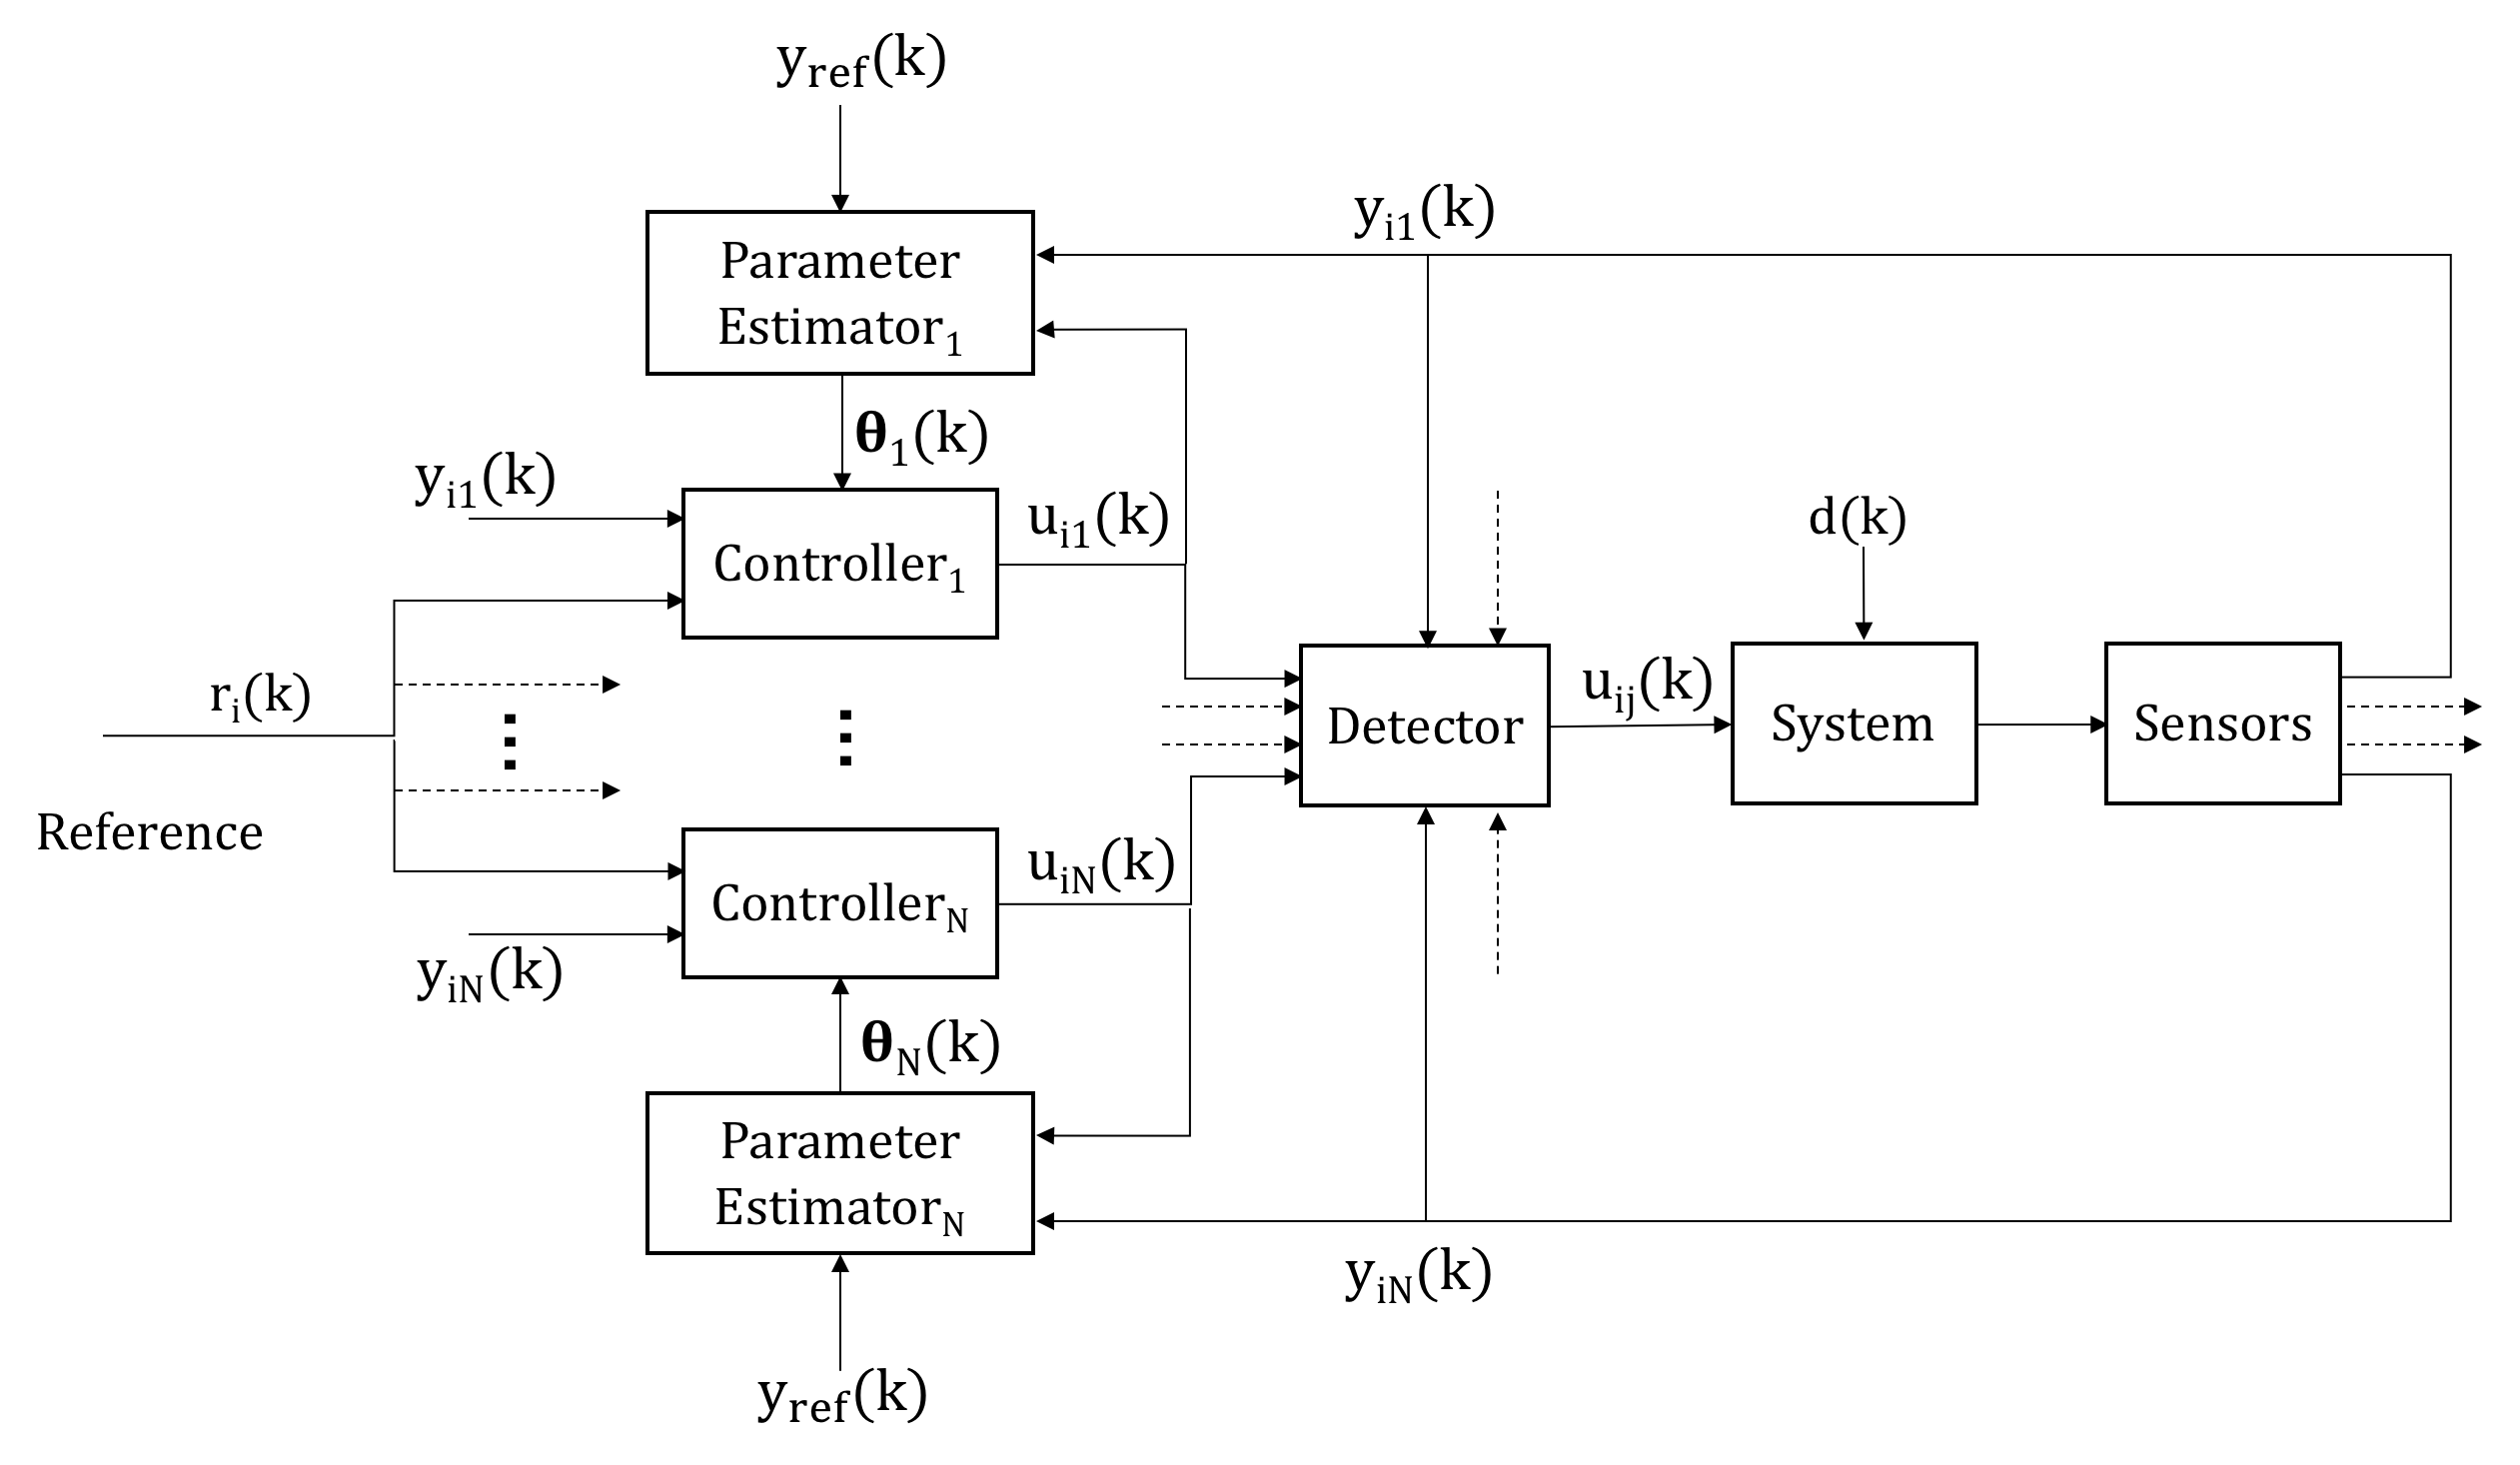
\includegraphics[width=0.48\textwidth]{con_and_det.png}
\caption{Architecture of the detection scheme within the adaptive controlled system. Representing  the $s$ number of available measurement sensors for that output.}
\label{fig:det_arch}
\end{figure}

To following equations \eqref{eq:Start}$-$\eqref{eq:End} will illustrate how to compute the input $u^*_i$ of each subsystem. Many steps to design the Characteristic Model Based all-coefficient Model Reference Adaptive Controller are omitted and can be found in \cite{tao2003adaptive,Goodwin1643720}, but we will emphasize the important equations. The model reference control is designed by solving the following polynomial equation,
%     \begin{equation}
%     \label{eq:Start}
% 	E(q^{-1})=F(q^{-1})A(q^{-1})+q^{-d}G(q^{-1})
% 	\end{equation}
% by matching the coefficients of $q^{-i}$ for both $F(q^{-1})$ and $G(q^{-1})$ with known polynomials $E(q^{-1})$ and $A(q^{-1})$ from \eqref{eq:E_q} and \eqref{eq:A_q}.
% Now, we express \eqref{eq:ARMA_equation_revise} as,
% 	\begin{equation}
% 	\label{eq:ARMA_equation_revise2}
% 	E(q^{-1})y_i(k+d)={\alpha}q^{-1}y_i(k) + {\beta}q^{-1}u_i(k)
% 	\end{equation}
% with the polynomials,
% 	\begin{equation}
% 	\alpha(q^{-1})=G(q^{-1})=\alpha_0+\alpha_1q^{-1}+ \dots +\alpha_{n-1}q^{-n+1}
% 	\end{equation}
% 	\begin{align}
% 	\begin{split}
% 	\beta( q^{-1})= F(q^{-1})&B^{'}(q^{-1})=\beta_0+\beta_1q^{-1} \\
% 	& + \dots +\beta_{m+d-1}q^{-m-d+1}, \beta_0\neq0
% 	\end{split}
% 	\end{align}
% The right side of equation \eqref{eq:ARMA_equation_revise2} can be expressed by para-metrization in the form,
%     \begin{equation}
% 	E(q^{-1})y_i(k+d)=\bm{\theta}_0(k)\bm{\phi}(k)
% 	\end{equation}
% with the unknown vector $\bm{\theta}_0$ and known signal vector $\bm{\phi}(k)$:
%     \begin{equation}
% 	\bm{\theta}_0=(\alpha_0, \dots ,\alpha_{n-1},\beta_0, \dots ,\beta_{m+d-1})^T \in \R^{n+m+d}
% 	\end{equation}
% 	\begin{align}
% 	\begin{split}
% 	\bm{\phi}(k)&=(y_i(k), \dots ,y_i(k-n+1),u_i(k), \dots , \\
% 	& u_i(k-m-d+1))^T \in \R^{n+m+d}
% 	\end{split}
% 	\end{align}
% Since we want the system to have the same characteristics as the reference model \eqref{eq:reference model_q}, we need to estimate the true parameter vector $\bm{\theta}_0$ with the estimated parameter vector $\bm{\theta}^T(k)$. 
%     \begin{equation}
%     \bm{\theta}(k)=(\theta_1(k), \dots ,\theta_n(k),\theta_{n+1}(k), \dots ,\theta_{n+m+d}(k))^T
% 	\end{equation}
% We update the estimate $\bm{\theta}^T(k)$ of the true parameter vector $\bm{\theta}_0$ using a \textit{Modified Projection Algorithm}:
% 	\begin{equation}
% 	\label{eq:Modified_Proj_Algorithm}
% 	\bm{\theta}(k)=\bm{\theta}(k-1)+\frac{a(k)\bm{\phi}(k-d)e(k)}{c+\bm{\phi}^T(k-d)\bm{\phi}(k-d)}
% 	\end{equation}
% 	\begin{equation}
% 	\bm{e}(k)=E(q^{-1})y_i(k)-\theta^T(k-1)\bm{\phi}(k-d)
% 	\end{equation}
% 	\begin{align*}
% 	\varepsilon<a(k)<2-\varepsilon, 0,\varepsilon<1, c>0
% 	\end{align*}
% To follow the desired tracking output $y^*(k)$ from the reference model, the adaptive control input $u(k)$ is then calculated from the equation:
%     \begin{equation}
%     \label{eq:tracking_model}
% 	\bm{\theta}^T(k)\bm{\phi}(k)=E(q^{-1})y_i^*(k+d)
% 	\end{equation}
% By rearranging \eqref{eq:tracking_model} we isolate $u(k)$ to calculate our next input signal for each subsystem:
% 	\begin{align}
% 	\label{eq:End}
% 	u_i(k)=\frac{1}{\theta_{n+1}(k)}&(-\theta_1(k)y_i(k)-\theta_2(k)y_i(k-1)  \nonumber \\
%     -\dots-\theta_n(k)y_i(k&-n-1)-\theta_{n+2}(k)u_i(k-1)  \\
% 	-\theta_{n+3}(k)u_i(k-2)-& \dots - \theta_{n+m+d}(k)u_i(k-m-d+1) \nonumber \\
% 	+g&H(q^{-1})r_i(k))^T \nonumber
% 	\end{align}
%     \begin{equation}
% 	\theta_{n+1}(k)\neq0 \nonumber
% 	\end{equation}




%%%%%%%%%%%%%%%%%%%%%% Beginning of Changes %%%%%%%%%%%%%%%%%%%%%

    \begin{equation}
    \label{eq:Start}
	E(z^{-1})=F(z^{-1})A(z^{-1})+z^{-d}G(z^{-1})
	\end{equation}
by matching the coefficients of $z^{-i}$ for both $F(z^{-1})$ and $G(z^{-1})$ with known polynomials $E(z^{-1})$ and $A(z^{-1})$ from \eqref{eq:E_q} and \eqref{eq:A_q}.
Now, we express \eqref{eq:ARMA_equation_revise} as,
	\begin{equation}
	\label{eq:ARMA_equation_revise2}
	E(z^{-1})y_i(k+d)={\alpha}z^{-1}y_i(k) + {\beta}z^{-1}u_i(k)
	\end{equation}
with the polynomials,
	\begin{equation}
	\alpha(z^{-1})=G(z^{-1})=\alpha_0+\alpha_1z^{-1}+ \dots +\alpha_{p-1}z^{-p+1}
	\end{equation}
	\begin{align}
	\begin{split}
	\beta( z^{-1})= F(z^{-1})&B^{'}(z^{-1})=\beta_0+\beta_1z^{-1} \\
	& + \dots +\beta_{q+d-1}z^{-q-d+1}, \beta_0\neq0
	\end{split}
	\end{align}
The right side of equation \eqref{eq:ARMA_equation_revise2} can be expressed by para-metrization in the form,
    \begin{equation}
	E(z^{-1})y_i(k+d)=\bm{\theta}_0(k)\bm{\phi}(k)
	\end{equation}
with the unknown vector $\bm{\theta}_0$ and known signal vector $\bm{\phi}(k)$:
    \begin{equation}
	\bm{\theta}_0=(\alpha_0, \dots ,\alpha_{p-1},\beta_0, \dots ,\beta_{q+d-1})^T \in \R^{p+q+d}
	\end{equation}
	\begin{align}
	\begin{split}
	\bm{\phi}(k)&=(y_i(k), \dots ,y_i(k-p+1),u_i(k), \dots , \\
	& u_i(k-q-d+1))^T \in \R^{p+q+d}
	\end{split}
	\end{align}
Since we want the system to have the same characteristics as the reference model \eqref{eq:reference model_q}, we need to estimate the true parameter vector $\bm{\theta}_0$ with the estimated parameter vector $\bm{\theta}^T(k)$. 
    \begin{equation}
    \bm{\theta}(k)=(\theta_1(k), \dots ,\theta_p(k),\theta_{p+1}(k), \dots ,\theta_{p+q+d}(k))^T
	\end{equation}
We update the estimate $\bm{\theta}^T(k)$ of the true parameter vector $\bm{\theta}_0$ using a \textit{Modified Projection Algorithm}:
	\begin{equation}
	\label{eq:Modified_Proj_Algorithm}
	\bm{\theta}(k)=\bm{\theta}(k-1)+\frac{a(k)\bm{\phi}(k-d)e(k)}{c+\bm{\phi}^T(k-d)\bm{\phi}(k-d)}
	\end{equation}
	\begin{equation}
	e(k)=E(z^{-1})y_i(k)-\theta^T(k-1)\bm{\phi}(k-d)
	\end{equation}
	\begin{align*}
	\varepsilon<a(k)<2-\varepsilon, 0,\varepsilon<1, c>0
	\end{align*}
To follow the desired tracking output $y^*(k)$ from the reference model, the adaptive control input $u(k)$ is then calculated from the equation:
    \begin{equation}
    \label{eq:tracking_model}
	\bm{\theta}^T(k)\bm{\phi}(k)=E(z^{-1})y_i^*(k+d)
	\end{equation}
By rearranging \eqref{eq:tracking_model} we isolate $u(k)$ to calculate our next input signal for each subsystem:
	\begin{align}
	\label{eq:End}
	u_i(k)=\frac{1}{\theta_{p+1}(k)}&(-\theta_1(k)y_i(k)-\theta_2(k)y_i(k-1)  \nonumber \\
    -\dots-\theta_p(k)y_i(k&-p-1)-\theta_{p+2}(k)u_i(k-1)  \\
	-\theta_{p+3}(k)u_i(k-2)-& \dots - \theta_{p+q+d}(k)u_i(k-q-d+1) \nonumber \\
	+g&H(z^{-1})r_i(k))^T \nonumber
	\end{align}
    \begin{equation}
	\theta_{p+1}(k)\neq0 \nonumber
	\end{equation}


%%%%%%%%%%%%%%%%%%%%%%%% End of Changes %%%%%%%%%%%%%%%%%%%%%%%%%%%



	
As shown in Fig. \ref{fig:det_arch}, each $i^{th}$ MRAC subsystem has its own measurement signal, but they all share the same reference model and input $u_i$ that is directly used to control the specific state. Each MRAC subsystem calculates an updated temporary input $u^*_i(k)$ that is fed into the detector, which analyses each $i^{th}$ input $u^*_i$ to check for attacks.

Since \eqref{multiple_output_tracking} should hold during any operation, the following is also true:
\begin{equation}
    \label{eq:u_to_0}
    \lim_{k\to\infty}(u^*_i(k)-u^*_j(k))=0, \text{ }i\neq j
\end{equation}
where $u^*_i$ and $u^*_j$ refer to temporary inputs calculated from their respected subsystems to control their measurement signal $y_i(k)$ towards the same tracking signal $y_i^*(k)$. Each temporary input, under ideal conditions, should be the same value as all other temporary inputs controlling their output to track the same tracking signal. For each subsystem to properly calculate the next input $u^*_i(k)$, their sensor measurement $y_i$ needs to be uncompromised. When one or more measurements have a non-zero value from the sensor attack vector $\xi_i(k) \neq 0$, those corresponding $i^{th}$ subsystem inputs $u^*_i$ diverge from the uncompromised subsystems.

For detection, a difference matrix $\Psi(k)$ is designed for every time interval $k$ of each controlled state. The structure of this matrix is,
    \begin{equation}
    \label{eq:error_matrix}
	\bm{\Psi}(k)=\begin{bmatrix} \psi_{1,1}(k) & \psi_{1,2}(k) & \dots & \psi_{1,s}(k) \\ \psi_{2,1}(k) & \psi_{2,2}(k) &  &  \\ \vdots &  & \ddots &  \\ \psi_{s,1}(k) &  &  & \psi_{s,s}(k) \end{bmatrix}
	\end{equation}
where $\bm{\Psi}(k) \in \R^{s\times s}$ with $s$ is the number of measurements from the available measurement set $\bm{y} \in \R^s$. Each element within $\bm{\Psi}(k)$ is represented as the absolute difference between two temporary inputs.
    \begin{equation}
        \psi_{i,j}(k)=|u^*_i(k)-u^*_j(k)|
    \end{equation}
We take an $l_1$ vector norm of the $i^{th}$ row from the difference matrix \eqref{eq:error_matrix} which gives us the following column vector:
    \begin{equation}
	\bm{\Psi^{'}}(k)=\begin{bmatrix} \lVert{\bm{\Psi}_1(k)}\rVert_1 \\ \lVert{\bm{\Psi}_2(k)}\rVert_1 \\ \vdots \\ \lVert{\bm{\Psi}_M(k)}\rVert_1 \end{bmatrix}
	\end{equation}
Next, another column vector $\bm{V}(k) \in \R^s$ is created with every element equal to $\min \bm{\Psi}^{'}(k)$:
    \begin{equation}
	\bm{V}(k)=\begin{bmatrix} \min \bm{\Psi}^{'}(k) & \min \bm{\Psi}^{'}(k) & \dots & \min \bm{\Psi}^{'}(k) \end{bmatrix}^T
	\end{equation}
We now define the error vector as:
    \begin{align}
    \label{eq:Psi2}
	\bm{\Psi^{''}}(k)&=\bm{\Psi^{'}}(k)-\bm{V}(k) \\
	& =\begin{bmatrix} \lVert{\bm{\Psi}_1(k)}\rVert_1 - \min \bm{\Psi}^{'}(k)\\ \lVert{\bm{\Psi}_2(k)}\rVert_1 - \min \bm{\Psi}^{'}(k) \\ \vdots \\ \lVert{\bm{\Psi}_M(k)}\rVert_1 - \min \bm{\Psi}^{'}(k) \end{bmatrix}
	\end{align}
	
From \eqref{eq:u_to_0} while under ideal conditions, the error vector \eqref{eq:Psi2} has all elements equal to zero. To constitute ideal conditions, uncertainties due to sensor and actuator noise, or any other unaccounted for changes to the state or measurement vectors are not considered. When an $i^{th}$ sensor is under attack, the $i^{th}$ input diverges from the remaining uncompromised inputs. The $i^{th}$ element of $\bm{\Psi}^{''}(k)$ becomes non-zero due to the compromised sensor, while the rest of the elements remain zero. 

Under non-ideal conditions where uncertainties exist, the elements of the error vector will not remain zero while sensors are uncompromised. By setting a threshold value $\delta$, we say all elements of the error vector need to stay below this level. By refining \eqref{eq:Psi2} for non-ideal conditions we get,
    \begin{align}
    \begin{split}
    \label{eq:Psi2_nonideal}
	\bm{\Psi^{''}}(k)&=\bm{\Psi^{'}}(k)-\bm{\Psi}(k) \\
	& =\begin{bmatrix} \lVert{\bm{\Psi}_1(k)}\rVert_1 - \min \bm{\Psi}^{'}(k)\\ \lVert{\bm{\Psi}_2(k)}\rVert_1 - \min \bm{\Psi}^{'}(k) \\ \vdots \\ \lVert{\bm{\Psi}_M(k)}\rVert_1 - \min \bm{\Psi}^{'}(k) \end{bmatrix} \leq \bm{\delta}
	\end{split}
	\end{align}
with the vector $\bm{\delta} \in \R^s$ has elements all equal to the scalar value $\delta$. When an $i^{th}$ element of $\bm{\Psi^{''}}(k)$ breaks the $\delta$ threshold, the corresponding $i^{th}$ measurement is placed into the set $\bm{y}_a$ for measurements no longer used by the system. The updated measurement set is $\bm{y}=\bm{y}_0\setminus\bm{y}_a$ where $\bm{y}_0$ was the initial full set of measurements and $\bm{y}_a$ is the set of removed measurements due to attacks. The updated measurement vector is of the dimensions $\bm{y} \in \R^{(s-s_{a})}$ with $s_a$ representing the size of set $\bm{y}_a$. The new updated dimensions of the output matrix due to the changing measurement vector is $\bm{C} \in \R^{(s-s_a)\times n}$. Effective detection is constrained to when less than of the measurements of the same controlled state are attacked. Once all temporary inputs $u_i^*(k)$ have been checked, the best available (e.g. measurement with lowest noise profile) is chosen to be used for the true control signal $u_i(k)$ to the system.



% DO I NEED THIS?

%Properties of the modified projection algorithm \eqref{eq:Modified_Proj_Algorithm} include:
%    \begin{enumerate}[label=(\roman*),leftmargin=3\parindent]
%	\item every iteration improves estimation:
%	    \begin{align}
%	        \|\bm{\theta}(k)-\bm{\theta}_0\|\leq\|\bm{\theta}(k-1)-\bm{\theta}_0\|, k\geq1 \nonumber
%	    \end{align}
%	\item parameter variation converges to zero:
%	    \begin{align}
%	        \lim_{k\to\infty}(\bm{\theta}(k)-\bm{\theta}(k-N))=0, \text{any finite } N>0 \nonumber
%	    \end{align}
%	\end{enumerate}
	
%(TALK ABOUT PERSISTENT EXCITATION BRIEFLY)
	

\subsection{Estimation Confidence}

In this work we leverage the statistical technique of confidence intervals \cite{devore2011probability} to obtain a specific confidence of an estimate. Confidence intervals are important because they calculate a confidence percentage that the true mean lies within the estimated bounds. As the number of data samples increases, the confidence interval shrinks in size to give a better estimation of the true mean. Assuming the knowledge of the confidence percentage $z^{*}$, population standard deviation $\sigma$, the number of sensor data samples $N$, and the mean of the $N$ sensor data samples $\bar{x}$, an interval of a percentage of confidence can be calculated:
    \begin{equation}
     \label{Confidence_interval}
		C_x = \bar{x} + z^{*}\frac{\sigma}{\sqrt{N}}
	\end{equation}
	
For position estimation with sensor uncertainties, we need a guarantee the vehicle is within a region to prevent navigation into an undesired state. To do this, uncompromised sensor measurements are fused using filtering techniques (e.g. Kalman Filtering) and the result is a position estimate $\hat{\bm{p}}=[\hat{x},\hat{y}]^T$ of a certain variance $\sigma_p^2$, which depends on the known sensor variances from data sheet specifications. Using an $N$ number of data samples of variance $\sigma_p^2$, we are able to estimate an interval of specific confidence that the vehicle is within the these boundaries.

For our case, we want to estimate a 2-dimensional interval. By calculating this multivariate confidence interval, we name it a confidence region, we estimate a region which the vehicle is within. This method guarantees the center of the vehicle has a specific percentage of confidence that it's within this region. The data being used for estimation has the form $\mathcal{N}(0,\sigma_p)$ where the position estimate data's population standard deviation $\sigma_p$ is known for any sensor combination. Using \eqref{Confidence_interval} we can find a multivariate region of a determined confidence percentage that the vehicle is within to ensure safety,
    \begin{equation}
    \label{Confidence_region}
		\hat{\bm{\varepsilon}}_{\hat{\bar{\bm{p}}}|N} = \hat{\bar{\bm{p}}} + c_p\frac{\sigma_p}{\sqrt{N}}
	\end{equation}
with $c_p$ defining the value for a specific confidence percentage, which can be found in $z$-tables and $t$-tables in \cite{devore2011probability}. The radius of the multivariate confidence region \eqref{Confidence_region} is:
    \begin{equation}
		\hat{\varepsilon} = c_p\frac{\sigma_p}{\sqrt{N}}
	\end{equation}
Similar to the calculation of confidence intervals, it is under the assumption the true mean is static, is not changing over time. This cannot be assumed in our case of position estimation of a navigating vehicle. 
\begin{figure}[ht!]
\vspace{1pt}
\centering
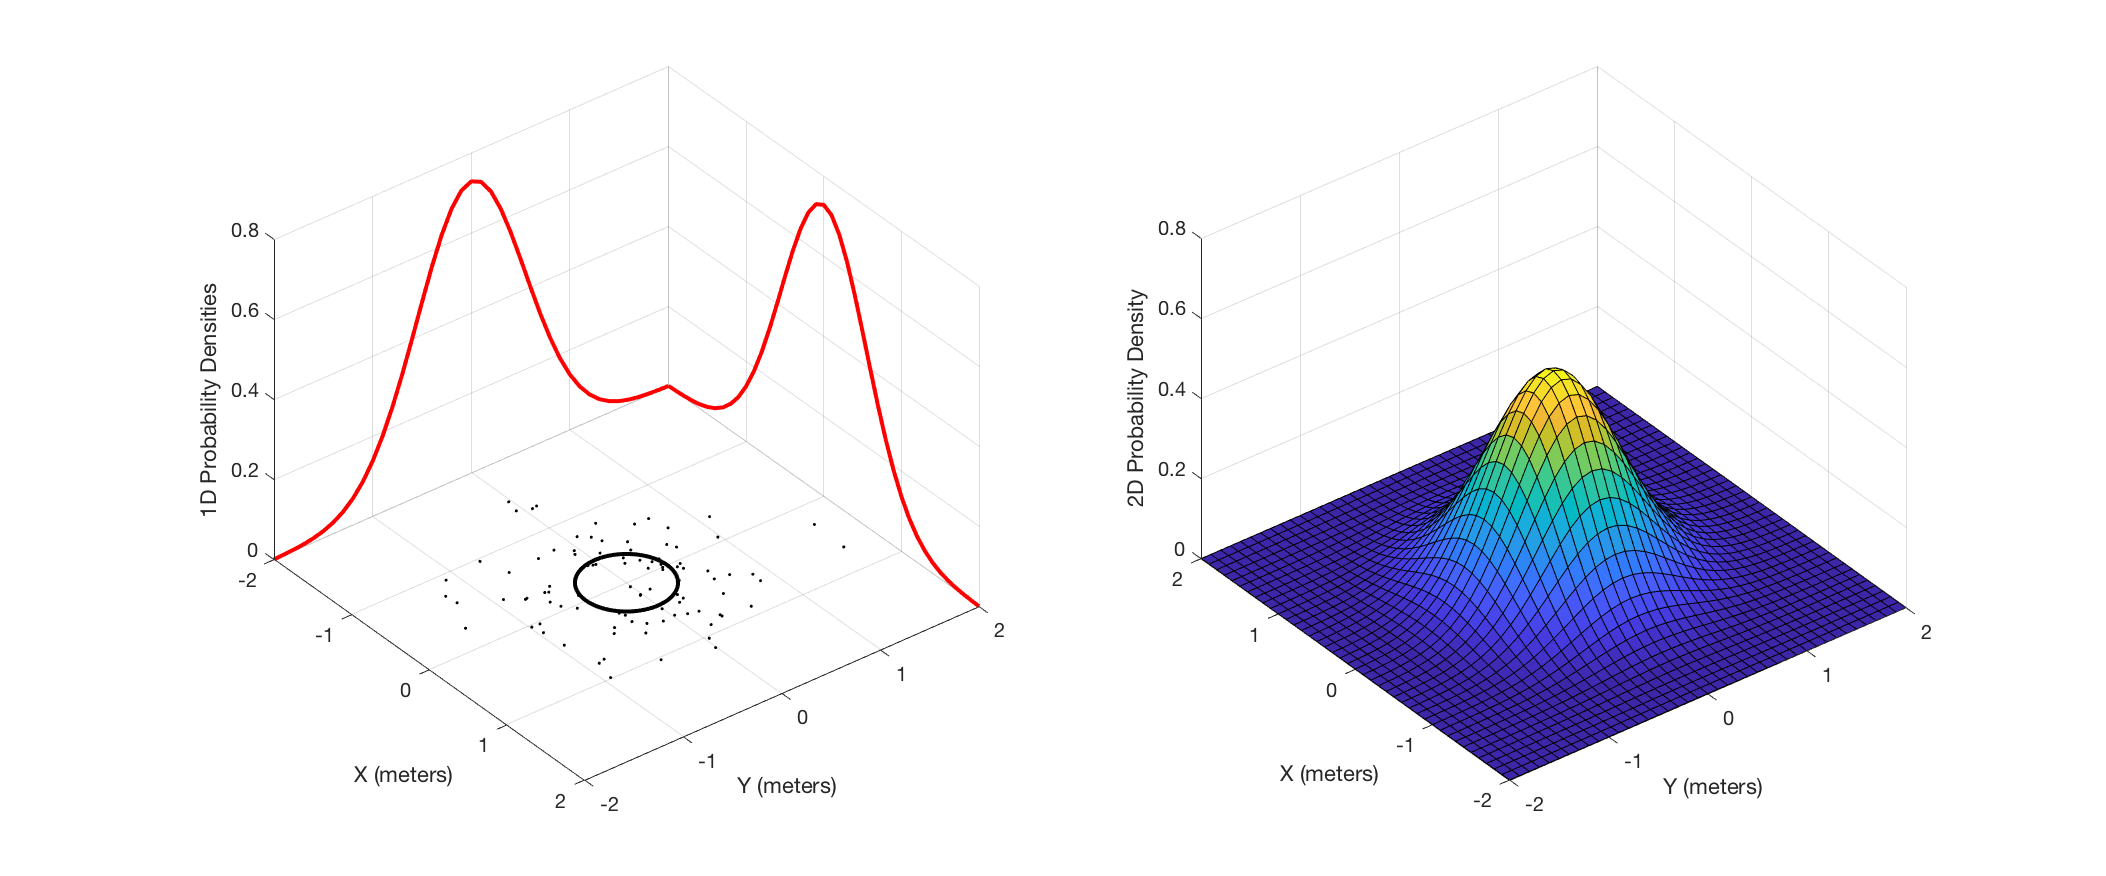
\includegraphics[width=0.48\textwidth]{Gaussian2D.png}
\caption{Distribution of vehicle's estimated position over 100 samples in an $X-Y$ plane with equal noise variance on the $X$ and $Y$ axis. Creating a psuedo-static case allows for the calculation of a confidence region for vehicle position.}
\label{fig:gauss_pdf}
\end{figure}

A pseudo-static form of a confidence region is made to compensate for translation of previous position measurements $\hat{\bm{p}}(k-i)$, where $i=1,2,\dots,N-1$. These $N-1$ number of previous position data points need to be represented as if they were all sampled for the current position in time $k$, creating a pseudo-static set of data to calculate the confidence region. As shown in Fig. \ref{fig:gauss_pdf}, we want to have the data samples for calculation of the confidence region look as if the vehicle is stationary. The $N$ position estimate samples are described in the set,
\begin{equation}
    \hat{\bm{P}}=\begin{bmatrix} \hat{\bm{p}}(k) ,\hat{\bm{p}}(k-1),\dots,\hat{\bm{p}}(k-N+1) \end{bmatrix} 
\end{equation}
for the position coordinates in the $x$ and $y$ direction. Translating the data coordinates into a pseudo-static form will create the updated set,
\begin{equation}
    \hat{\bm{P}}^*=\begin{bmatrix} \hat{\bm{p}}^*(k) ,\hat{\bm{p}}^*(k-1),\dots,\hat{\bm{p}}^*(k-N+1) \end{bmatrix} \nonumber
\end{equation}
Each element of these updated sets are calculated as,
	\begin{equation}
	\hat{\bm{p}}^*(k-i) = \hat{\bm{p}}(k-i)+\sum_{j=i}^1 v(k-j)\theta_h(k-j)t_s 
	\end{equation}
where $i=1,2,\dots,N-1$ and the most recent position estimate at time instant $k$ is unchanged from $\hat{\bm{p}}(k)$ to $\hat{\bm{p}}^*(k)$. The mean of the updated set is written as $\hat{\bar{\bm{p}}}^*$, which is used for the calculation of the estimated confidence region. To demonstrate how this works, Fig. \ref{fig:pseudo_static} gives a visualization of how the position estimates are transitioned into a pseudo-static case. Updating \eqref{Confidence_region}, we get
    \begin{equation}
    \label{Confidence_region_updated}
		\hat{\bm{\varepsilon}}_{\hat{\bar{\bm{p}}}^*|N} = \hat{\bar{\bm{p}}}^* + C_p\frac{\sigma_p}{\sqrt{N}}
	\end{equation}
 to account for all $N-1$ translated previous data points to appear as if they all were sampled at time interval $k$.

\begin{figure}[ht!]
\vspace{1pt}
\centering
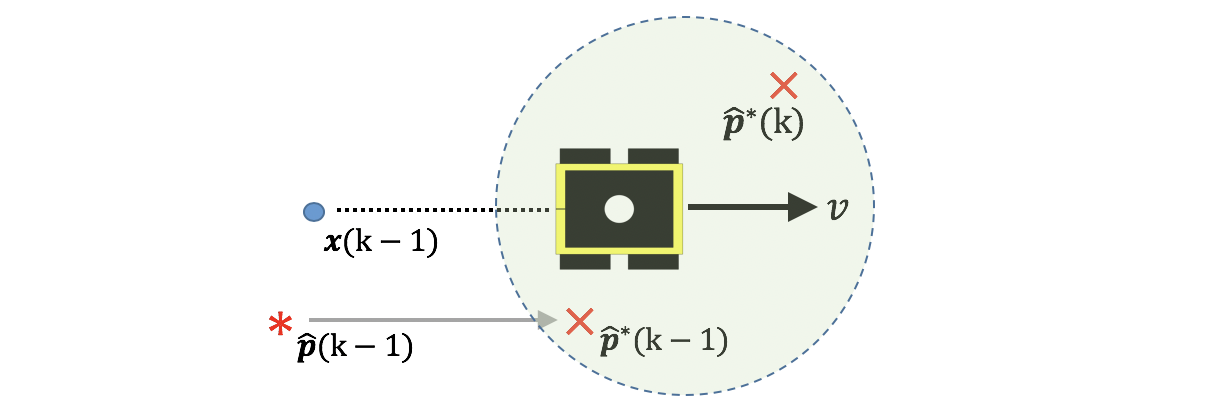
\includegraphics[width=0.48\textwidth]{pseudo_static.png}
\caption{Translation of the original position estimates $\hat{\bm{p}}(k)$ to a pseudo-static case $\hat{\bm{p}}^*(k)$ as if all the position estimates were sampled from the vehicle at the current time $k$.}
\label{fig:pseudo_static}
\end{figure}

Creating a pseudo-static case with these past position data samples introduces higher uncertainty. Uncertainties regarding the velocity sensor $\sigma_v$ and heading angle sensor $\sigma_h$ need to be accounted for. To guarantee the true position of the vehicle is within the estimation radial bounds, the maximum error in position due to the actuator and sensor noises over the furthest sample in time in $\hat{\bm{P}}^*$ is calculated as:
    \begin{equation}
	\hat{\varepsilon}_{v,\theta_h|N}^{*}=\sqrt{(v^{*}\cos{\theta_h^{*}})^2+(v^{\star}\sin{\theta_h^{*}})^2} \cdot Nt_s
	\end{equation}
where,
    \begin{equation}
	v^{*}=\bar{v}(k-i_{\varepsilon^{*}})+c_p\sigma_v \nonumber
	\end{equation}
	\begin{equation}
	\theta_h^{*}=\bar{\theta}_h(k-i_{\varepsilon^{*}})+c_p\sigma_h \nonumber
	\end{equation}
with $i_{\varepsilon^{*}}=[1,2,,\dots,N]$ while average measured velocity and average measured heading angles over the past $N$ samples are denoted by $\bar{v}$ and $\bar{\theta}_h$, respectively. Doing this account for velocity and heading angle measurement error and ensure the vehicle's position is within our estimation region.


\subsection{Adaptive Motion Planning}
With uncertainty of sensor measurements, with or without the loss of a compromised sensors, there needs to be guarantees to safely navigate a vehicle without accidents. As the vehicle approaches undesired regions or has a trajectory to follow through a passageway that's more narrow than the confidence region at the current time interval $k$, we need to be able to reduce the size of estimate region to guarantee safety. The only two options are to sample data faster or reduce speed to gather more samples within a certain distance. Since sampling at a faster rate can't be done, we need to slow the vehicle down to gather more data samples in a shorter distance to reduce estimation uncertainties.

To keep the vehicles estimated confidence region from intersecting with an unwanted region, a change to the number of current and past data samples in the calculation as well as an adaptation of the velocity. Without uncertainty of velocity and heading angle measurements, the equation to solve for the number of required $N$ samples to keep the confidence region within a specific radius is:
    \begin{equation}
    \label{conf_region1}
	    N^* = \left(c_p \frac{ \sigma_p }{ {\min \lVert \bm{x}_r - \hat{\bar{\bm{p}}}^* \rVert} -\Delta(k) } \right)^2
	\end{equation}
where $ \min \lVert {\bm{x}_r-\hat{\bar{\bm{p}}}^*} \rVert$ is the distance from the closest undesired region to the estimated vehicle center point position $\hat{\bar{\bm{p}}}^*$.
With the assumption of Normally distributed sensor noise on the velocity and heading angle sensors, the above equation is not suitable. The uncertainty region $\hat{\varepsilon}_{v,\theta_h|N}^{*}$ from these sensors must be accounted for. The revision to equation (\ref{conf_region1}) for a sufficient value of $N$ is:
    \begin{equation}
	    N^* = \left(c_p \frac{ \sigma_p }{ {\min \lVert \bm{x}_r - \hat{\bar{\bm{p}}}^* \rVert} -\hat{\varepsilon}_{v,\theta_h|N}^{*}-\Delta(k) } \right)^2
	\end{equation}
Due to the fact that $N^*$ represents the number of samples needed to reduce the estimation region to a desired size, $N^*$ needs to be an integer. We simply round $N^*$ up to the nearest integer to give us $N \in \N$.

An update of the reference velocity needs to occur when these undesired regions are within the entire confidence estimation region $ \hat{\varepsilon}_{\hat{\bar{\bm{p}}}^*|N} +\hat{\varepsilon}_{v,\theta_h|N}^{*}+\Delta(k)$ when $N=1$ to ensure the vehicle slows to capture more previous data samples with less estimation error. This reference velocity $r_v(k)$ update is calculated by:
    \begin{equation}
	    r_v(k)=r_v(k-1) \left[ \frac{ \min \lVert \bm{x}_r - \hat{\bar{\bm{p}}}^* \rVert - \hat{\varepsilon}_1}{\hat{\varepsilon}_2 - \hat{\varepsilon}_1} \right]
	\end{equation}
	\begin{equation}
	\begin{split}
	    \hat{\varepsilon}_1&=\hat{\bm{\varepsilon}}_{\hat{\bar{\bm{p}}}^*|N} +\hat{\varepsilon}_{v,\theta_h|N}^{*},\\ &\hat{\varepsilon}_2=\hat{\varepsilon}_1+\Delta(k) \nonumber	    
	\end{split}
	\end{equation}
	
where $\hat{\varepsilon}_1$ and $\hat{\varepsilon}_2$ are both radii from the estimated center position $\hat{\bar{\bm{p}}}^*$.
	
%	\begin{equation}
%		\Delta(k)=[v(k)]^{\delta_v}\delta
%	\end{equation}
%where $[\delta, \delta_v] \in R^{\geq0}$ are chosen values that determine the desired distance between the closest unwanted region to the estimation region as a function of velocity.


% INSERT ALGORITHM FOR REPLANNING VELOCITY
\begin{algorithm}
   \caption{Adaptive Motion for Safe Navigation} 
   \label{alg:adapt_motion} 
    \begin{algorithmic}[1]
	\State Initial conditions of system: $k=0$,$\bm{x}(0)=\bm{x}_0$
	\State Set $r_v(0)$ to desired velocity $r_{des}$
    \While{$1<k\leq\infty$}
        \State \Longunderstack[l]{ Calculate $\hat{\bar{\bm{p}}}^*$ then measure closest distance\\ to undesired region $\min \lVert \bm{x}_r - \hat{\bar{\bm{p}}}^* \rVert$.}
        \State Calculate radii of intervals $\hat{\varepsilon}_1$ and $\hat{\varepsilon}_2$ for $N$.
        \If{ $\min \lVert \bm{x}_r - \hat{\bar{\bm{p}}}^*\rVert < \hat{\varepsilon}_2(k)$}
            \State Solve for $N$ of next iteration
            \State Update reference for velocity $r_v(k)$
        \Else
            \If{$\min \lVert \bm{x}_r - \hat{\bar{\bm{p}}}^*\rVert < \hat{\varepsilon}_2(k)$ when $N=1$}
                \State Solve for $N$ of next iteration
                \State Update reference for velocity $r_v(k)$
            \Else
                \If{$r_v(k) \neq r_{des}$}
                    \State Reference velocity $r_v(k)=r_{des}$
                    \State $N = 1$
                \Else
                    \State Reference velocity $r_v(k) = r_v(k-1)$
                    \State $N = 1$
                \EndIf
            \EndIf
        \EndIf
    \EndWhile
	\end{algorithmic}
\end{algorithm}



\end{section} 